 	
\documentclass[12pt]{article}
\usepackage{amsfonts,amsmath,amssymb,amsthm}
\usepackage{bm}
\usepackage{enumerate}
\usepackage{enumitem}
\usepackage{graphicx}
\graphicspath{{images/}}
\usepackage{multirow}
\providecommand{\abs}[1]{\lvert#1\rvert}
\providecommand{\norm}[1]{\lVert#1\rVert}

\newtheorem{hw}{Problem}
\newenvironment{sol}
{\par\vspace{3mm}\noindent{\it Solution}.}
{\qed}

% Create automatically bolded vectors
\let\oldhat\hat
\renewcommand{\vec}[1]{\bm{\mathrm{#1}}}
\renewcommand{\hat}[1]{\oldhat{\bm{#1}}}

\setlength{\parindent}{0pt}
%\setlength{\parskip}{2ex}
\newenvironment{proofof}[1]{\bigskip\noindent{\itshape #1. }}{\hfill$\Box$\medskip}

\usepackage{enumerate,fullpage,proof}
\usepackage{subfigure}
\usepackage{graphicx}
\newcommand{\Infer}[2]{\infer{#2}{#1}}

\begin{document}
	
	$\;$\hfill Due: 2018/05/21
	
	\begin{center}
		{\LARGE\bf Machine Learning: Homework 5}
	\end{center}
	
	\textbf{Student Number:}
	
	\textbf{Name:}
	
    
\begin{hw}\rm
Use the  k-means algorithm and Euclidean distance to cluster the following 8 examples into 3 clusters: $A_1 = (2,10)$, $A_2 = (2,5)$, $A_3 = (8,4)$, $A_4 = (5,8)$, $A_5 = (7,5)$, $A_6 = (6,4)$, $A_7 = (1,2)$, $A_8 = (4,9)$. The distance matrix based on the Euclidean distance is given below:
\begin{table}
\begin{center}
\begin{tabular}{ |c|c|c|c|c|c|c|c|c| } 
 \hline
 & $A_1$ & $A_2$ & $A_3$ & $A_4$ & $A_5$ & $A_6$ & $A_7$ & $A_8$\\ 
  \hline
 $A_1$ & 0 & $\sqrt{25}$ & $\sqrt{36}$ & $\sqrt{13}$ & $\sqrt{50}$ & $\sqrt{52}$ & $\sqrt{65}$ & $\sqrt{5}$\\ 
  \hline
 $A_2$ & & 0 & $\sqrt{37}$ & $\sqrt{18}$ & $\sqrt{25}$ & $\sqrt{17}$ & $\sqrt{10}$ & $\sqrt{20}$\\ 
  \hline 
 $A_3$ & & & 0 & $\sqrt{25}$ & $\sqrt{2}$ & $\sqrt{2}$ & $\sqrt{53}$ & $\sqrt{41}$\\ 
  \hline
 $A_4$ & & & & 0 & $\sqrt{13}$ & $\sqrt{17}$ & $\sqrt{52}$ & $\sqrt{2}$\\
  \hline 
 $A_5$ & & & & & 0 & $\sqrt{52}$ & $\sqrt{65}$ & $\sqrt{5}$\\ 
  \hline
 $A_6$ & & & & & & 0 & $\sqrt{65}$ & $\sqrt{5}$ \\ 
  \hline
 $A_7$ & & & & & & & 0 & $\sqrt{5}$ \\ 
  \hline
 $A_8$ & & & & & & & & 0 \\ 
 \hline
\end{tabular}
\end{center}
\end{table}
Suppose that the initial seeds (centres of each cluster) are $A_1$, $A_4$ and $A_7$. Run the k-means algorithm for
1 epoch only. At the end of this epoch show:
\begin{enumerate}[label=(\alph*)]
\item The new clusters (i.e. the examples belonging to each cluster).
\item The centres of the new clusters.
\item Draw a 10 by 10 space with all the 8 points and show the clusters after the first epoch and the new
centroids.
\end{enumerate}

\end{hw}   
	\begin{center}
		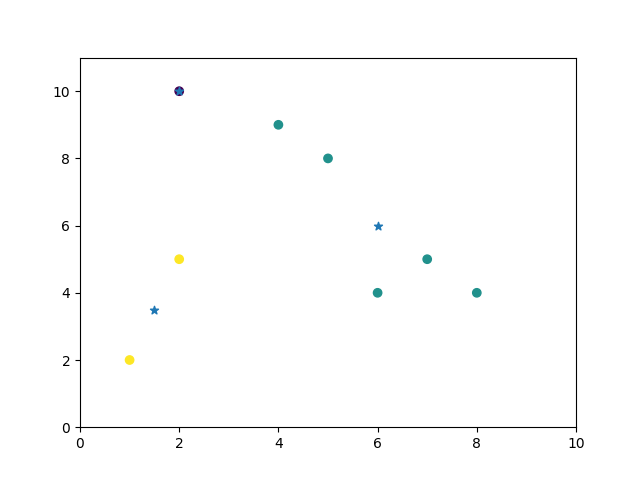
\includegraphics[angle = 0, width = .8\textwidth]{./images/fig6.png}
	\end{center}
	The code is available on my github https://github.com/sunyasheng/.\\
\begin{proofof}a
 	The new clusters are represented with different colors as is shown in figure above.
\end{proofof}

\begin{proofof}b
	The centers of new clusters is represented by stars. Their coordinates are [2.0, 10.0], [6.0, 6.0], [1.5, 3.5].
\end{proofof}

\begin{proofof}c
	The clusters and centeroids are shown in the figure above in 11 by 10 space. 
\end{proofof}

\begin{hw}\rm
Assume we are given n points $\{x^1,\dots,x^n\}\in X^n $.\\
Let $k : X \times X \rightarrow R$ be a kernel, with the corresponding feature map $\phi : X \rightarrow H$. We denote by K the $n\times n$ matrix such that $K_{ij} = k(x^i,y^j)$. We denote by $\sigma$ the sample covariance matrix of the images $\{ \phi(x^1),\dots,\phi(x^n)\}$ of our data. Let $\lambda$ and V be an eigenvalues and corresponding eigenvector of $\sigma$.
\begin{enumerate}[label=(\alph*)]
\item Write $k(x,x^{'})$ as a function of $\phi(x)$ and $\phi(x^{'})$.
\item Show that V is a linear combinations of $\{ \phi(x^1),\dots,\phi(x^n)\}$.
\item We can now write $V = \sum^n_{i=1} \alpha_i \phi(x^i)$. Let us denote by $\alpha$ the n-dimensional vector $(\alpha_1, \dots, \alpha_n)$. Show that $\lambda$, V are solution to $n\lambda K \alpha = K^2 \alpha$.
\item 
Show how PCA in the feature space can be conducted directly in the orignal space X, using only k and never computing $\phi(x)$ for any x
\item What is the advantage of never having to compute $\phi(x)$ explicitly?
\item Can you get an explicit expression of the principal components without using $\phi$?
\end{enumerate}
\end{hw}

\begin{proof}
\begin{enumerate}[label=(\alph*)]
\item
\begin{align*}
	k(x, x') = \Phi(x)^T\Phi(x')
\end{align*}
\item
\begin{align*}
	\frac{1}{n} \Sigma V = \frac{1}{n} \Phi \Phi^T V = \frac{1}{n} \Phi \beta = \lambda V \\
	V = \frac{1}{n \lambda} \Phi \beta
\end{align*}
\item
\begin{align*}
	\frac{1}{n} \Sigma V = \frac{1}{n} \Phi \Phi^T V = \frac{1}{n} \Phi \Phi^T \Phi \alpha = \lambda V = \lambda \Phi \alpha\\
	\frac{1}{n} \Phi^T \Phi \Phi^T \Phi \alpha = \lambda \Phi^T \Phi \alpha \\
	K^2 \alpha = n \lambda K \alpha
\end{align*}
\item
Following the previous equation, the $\alpha$ can be solved. Fomally,
$$V = \Phi \alpha$$
The dot product between $V$ and any $\Phi(x)$ can be achieved by 
$$\Phi(x)^T V = \Phi(x)^T \Phi \alpha = K(x, x') \alpha$$
\item
The feature space might be a huge space or even infinite space. The compuatation of mapping function is unrealisic. 
\item
$$V = \Phi \alpha$$\\
Explicit impression without usage of $\Phi$ is difficult.

\end{enumerate}
\end{proof}

\begin{hw}\rm
Consider a random variable x that is categorical with M possible values $1, \dots, M$. Suppose x is represented as a vector such that $x(i) = 1$ if x takes the ith value, and $\sum_i x(i) = 1$.The distribution of x is described by a mixture of K discrete Multinomial distributions such that
\begin{align*}
	p(x) = \sum_{k=1}^K \pi_k p(x|\mu_k)
\end{align*}
and
\begin{align*}
	 p(x|\mu_k) = \prod_{j=1}^M\mu_k(j)^{x(j)}
\end{align*}
where $\pi_k$ denotes the mixing coefficient for the kth component (aka the prior probability that the hidden variable z = k), and $\mu_k$ specifies the parameters of the kth component. Specifically, $\mu_k(j)$ represents the probabilities $p(x(j) = 1|z = k)$, and $\sum_j µ_k(j) = 1$. Given an observed
data set {xi}, $i = 1, \dots , N$, please derive the E and M step equations of the EM algorithm for optimizing the mixing coefficient and the component parameters $\mu_k(j)$ for this distribution.
\end{hw}

\begin{proof}
E-step:
	\begin{align*}
		<k\mid x> = p(k\mid x_i) = \frac{p(k, x_i)}{\sum_{k=1}^{K}p(k,x_i)} = \frac{\pi_k \prod_{j=1}^{M} \mu_k(j)^{x_i(j)}}{\sum_{k=1}^K \pi_k \prod_{j=1}^{M} \mu_k(j)^{x_i(j)}}
	\end{align*}
M-step:
	\begin{align*}
		\frac{\partial \sum_{k=1}^K <k\mid x> (lg \pi_k + p(x\mid \mu_k))}{\partial \pi_k} = 0 \\
		\pi_k \sim <k \mid x> \\
		\pi_k =  \frac{<k>}{N}
	\end{align*}
	\begin{align*}
		\frac{\partial \sum_{k=1}^K <k\mid x> (lg \pi_k + p(x\mid \mu_k))}{\partial \mu_k} = 0 \\
		\mu_k(j) \sim <k \mid x> x_i(j) \\
		\mu_k(j) =  \frac{<k \mid x> x_i(j)}{\sum_{j=1}^M <k \mid x> x_i(j)}
	\end{align*}
\end{proof}
 

\end{document}

